
% License:
% CC BY-NC-SA 3.0 (http://creativecommons.org/licenses/by-nc-sa/3.0/)
%
%%%%%%%%%%%%%%%%%%%%%%%%%%%%%%%%%%%%%%%%%

%----------------------------------------------------------------------------------------
%	PACKAGES AND OTHER DOCUMENT CONFIGURATIONS
%----------------------------------------------------------------------------------------

\documentclass[paper=a4, fontsize=11pt]{scrartcl} % A4 paper and 11pt font size

\usepackage[T1]{fontenc} % Use 8-bit encoding that has 256 glyphs
\usepackage{fourier} % Use the Adobe Utopia font for the document - comment this line to return to the LaTeX default
\usepackage[english]{babel} % English language/hyphenation
\usepackage{amsmath,amsfonts,amsthm} % Math packages
\usepackage{lipsum} % Used for inserting dummy 'Lorem ipsum' text into the template

\usepackage{caption}
\usepackage{subcaption}
\usepackage{graphicx}
\usepackage{listings}
\usepackage[table,xcdraw]{xcolor}


\usepackage{float}

\usepackage{blindtext} %for enumarations

\usepackage[]{hyperref}  %link collor

%talbe layout to the right
\usepackage[labelfont=bf]{caption}
\captionsetup[table]{labelsep=space,justification=raggedright,singlelinecheck=off}
\captionsetup[figure]{labelsep=quad}

\usepackage{sectsty} % Allows customizing section commands
\allsectionsfont{\raggedright \normalfont\scshape} % Make all sections centered, the default font and small caps

\usepackage{fancyhdr} % Custom headers and footers
\pagestyle{fancyplain} % Makes all pages in the document conform to the custom headers and footers
\fancyhead{} % No page header - if you want one, create it in the same way as the footers below
\fancyfoot[L]{} % Empty left footer
\fancyfoot[C]{} % Empty center footer
\fancyfoot[R]{\thepage} % Page numbering for right footer
\renewcommand{\headrulewidth}{0pt} % Remove header underlines
\renewcommand{\footrulewidth}{0pt} % Remove footer underlines
\setlength{\headheight}{13.6pt} % Customize the height of the header

\numberwithin{equation}{section} % Number equations within sections (i.e. 1.1, 1.2, 2.1, 2.2 instead of 1, 2, 3, 4)
\numberwithin{figure}{section} % Number figures within sections (i.e. 1.1, 1.2, 2.1, 2.2 instead of 1, 2, 3, 4)
\numberwithin{table}{section} % Number tables within sections (i.e. 1.1, 1.2, 2.1, 2.2 instead of 1, 2, 3, 4)

%\setlength\parindent{0pt} % Removes all indentation from paragraphs - comment this line for an assignment with lots of text


\setlength\parskip{4pt}

%----------------------------------------------------------------------------------------
%	TITLE SECTION
%----------------------------------------------------------------------------------------

\newcommand{\horrule}[1]{\rule{\linewidth}{#1}} % Create horizontal rule command with 1 argument of height

\title{	
\normalfont \normalsize 
\textsc{Saturdays AI, Jalisco} \\ [25pt] % Your university, school and/or department name(s)
\horrule{0.5pt} \\[0.4cm] % Thin top horizontal rule
\huge  Brecha Salarial de G\'enero en M\'exico: An\'alisis y Predicci\'on con Machine Learning de la Tendencia en 2019\\ % The assignment title
\horrule{2pt} \\[0.5cm] % Thick bottom horizontal rule
\textsc{WageForecasterMX} \\ [25pt]
}


\author{  Lara Pacheco,Erick Alberto \\ Bello Monzoy, Jos\'e Alfredo \\ Mart\'in del Campo G\'omez, Anah\'i \\ Cedillo Padilla, Xochitl Alejandra \\ Torres Naranjo, Silvia Leticia \\ Mendoza Carlos} % Your name

\date{\normalsize\today} % Today's date or a custom date

\begin{document}
%\nocite{*}
\maketitle % Print the title

\newpage
\begin{abstract}

{\noindent{\Large Abstract} }\\
A pesar de que actualmente muchas de las mujeres se encuentran igualdad de formaci\'on y experiencia, diferentes organismos han demostrado que existe una gran brecha salarial de g\'enero en el Mundo. Tan solo en Am\'erica Latina, México es el pa\'s con la peor brecha salarial, seg\'un public\'o Forbes en un informe de julio de 2019. Dada la actual situac\'on en M\'exico y la agenda que el pa\'is tiene para reducir esta brecha surgen preguntas tales como: `` ?` Qu\'e variables en M\'exico tienen mayor influencia en el salario? ?`Es diferente seg\'un el g\'enero?''.
\\El presente trabajo tiene como objetivo generar un modelo, usando m'etodos no lineales, que permita calcular el salario usando variables como el estado, g\'enero y rango de edades. La intenci\'on es que las predicciones generadas por el modelo sean utilizadas por organizaciones y que ayuden a tomar decisiones informadas en la implementaci\'on de pol\'iticas p\'ublicas estrat\'egicas para disminuir la brecha salarial entre hombres y mujeres.
\\
\\
\textbf{Key words:} Machine Learning, Algoritmos de regresi\'on, Brecha salarial de G\'enero, Wage Forecast
    
\end{abstract}

\newpage
\tableofcontents

%----------------------------------------------------------------------------------------
%	Section 1
%----------------------------------------------------------------------------------------
%how to cite
%\cite{Seow2011}
%how to add figure
%\ref{fig:TotalConsumption} 

%\begin{figure}[h!]
%	\centering
%	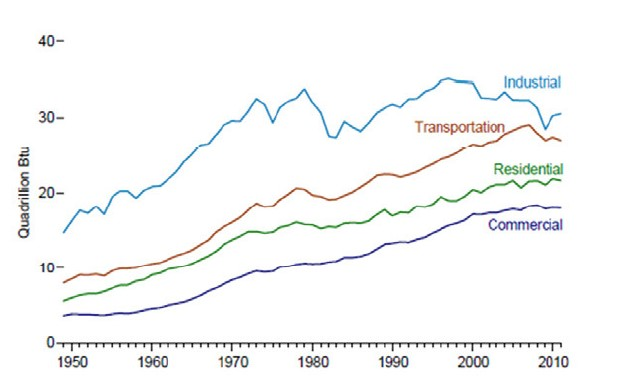
\includegraphics[width=0.8\linewidth]{Figure/Total-consumption.jpg}
%	\caption{Total Consumption by End-Use Sector, 1949-2011 
%   \cite{Apostolos2013}}
%	\label{fig:TotalConsumption}
%\end{figure}



\newpage
\section{Introducci\'on}
\label{chapter1}
%\textit{Person in Charge; }

\subsection{}




%----------------------------------------------------------------------------------------
%	Section 2
%----------------------------------------------------------------------------------------
\newpage
\section{Marco Te\'orico}

\subsection{Estudios Actuales}
Las brechas salariales de g\'enero en M\'exico se han estudiado asiduamente. Entre los primeros an\'alisis de las brechas salariales se encuentra el de (Alarc\'on, 1994), quienes utilizaron la muestra urbana de la Encuesta Nacional de Ingreso y Gasto de los Hogares (ENIGH) de 1984, 1989 y 1992. En sus trabajos encontraron que en 1984 las mujeres ganaban 23.3\% menos que los hombres; hacia 1989 esta cifra hab\'ia aumentado a 28.4\%, y en 1992 disminuy\'o a 25.3\%. Siguiendo la l\'inea de investigaci\'on de Oaxaca (1973) y Blinder (1973), estos autores realizaron una descomposici\'on de la brecha salarial en la media, mediante la estimaci\'on de ecuaciones de Mincer (1974) , para analizar tanto la parte de la brecha originada por caracter\'isticas observables como la parte provocada por los retornos a tales caracter\'isticas. Encontraron tambi\'en que s\'olo 27.5\% de la brecha se explicaba por diferencias en capital humano en 1984, mientras que en 1989 la proporci\'on fue de 14.4\% y en 1992 de 21.2\%; es decir que entre 70 y 85\% de las brechas se deb\'ian a diferencias en los retornos al capital humano, lo cual podr\'ia sugerir discriminaci\'on en contra de las mujeres o diferencias en productividad que no fueron controladas en la regresi\'on.

Por su parte, Brown, Pagan y Rodr\'iguez-Oreggia (1999) analizaron los cambios en las brechas salariales entre 1987 y 1993 con base en datos de los terceros trimestres de la Encuesta Nacional de Empleo Urbano. Ellos realizaron una descomposici\'on de Wellington (1993) de los cambios de la brecha en el tiempo, y una descomposici\'on de Oaxaca-Blinder para analizar el efecto de la estructura ocupacional en la brecha. Encuentran que la brecha creci\'o en el periodo de un nivel inicial de 20.8\%, en 1987, a 22\%, en 1993. Este crecimiento en la brecha se debi\'o a cambios en las dotaciones, pues a causa de los cambios en los retornos la brecha se hubiese cerrado. Los autores tambi\'en encontraron que la mayor parte de la brecha se gener\'o por diferencias en retornos. Sin embargo, lo interesante de sus hallazgos es que la inclusi\'on de controles ocupacionales aumenta la proporci\'on de la brecha explicada por diferencias a los retornos, lo cual, seg\'un explican, puede ser resultado de la poca desagregaci\'on de las categor\'ias ocupacionales. Es decir, la segregaci\'on ocupacional disminuye la brecha salarial en M\'exico, lo cual contrasta con los resultados de otros pa\'ises (Blau, Simpson y Anderson, 1998).

M\'as recientemente, Pagan y Ullibarri (2000) analizaron la desigualdad salarial entre hombres y mujeres por medio del \'indice de Jenkins, corrigiendo por selecci\'on en la participaci\'on laboral de las mujeres. Con base en datos de la ENEU del tercer trimestre de 1995, encontraron que existe mayor desigualdad entre personas con alta y baja escolaridad, as\'i como entre aquellas con mayor experiencia. Por su parte, elaboraron una descomposici\'on del tipo Oaxaca-Blinder mediante la ENIGH 2000, corrigiendo por sesgo de selecci\'on con la metodolog\'ia de Heckman (1974, 1979). Los autores fueron los primeros en incluir en su an\'alisis zonas urbanas y rurales. Hallaron que 85\% de la brecha se debe a diferencias en retornos y que \'esta es mayor en zonas rurales; de hecho, el efecto de las dotaciones otorga una ventaja a las mujeres. Por \'ultimo, Garc\'ia y Mendoza (2009) elaboraron una descomposici\'on de Oaxaca-Blinder sin corregir por sesgo de selecci\'on y usando datos de la ENOE 2006. Su hallazgo fue una brecha salarial de 12.4\% y, al contrario que el resto de la bibliograf\'ia, determinaron que 87.6\% de la brecha se explica por diferencias en las dotaciones, seg\'un la cual el 12.4\% restante corresponde a diferencias en los retornos a \'estas.

\subsection{An\'alisis desde el Contexto Social}
Para el caso de M\'exico, la \'unica causa explorada de la brecha no explicada o la brecha de retornos ha sido la liberalizaci\'on comercial Artecona y Cunningham (2002) encuentran evidencia que sugiere que la liberalizaci\'on comercial provoc\'o una disminuci\'on de la discriminaci\'on en las empresas manufactureras que fueron más afectadas por la liberalizaci\'on. Por su parte, Aguayo-T\'ellez, Airola y Juhn (2010) encuentran que la liberalizaci\'on comercial no afect\'o los salarios, pero s\'i tuvo un efecto en el empleo de las mujeres. De esta manera, la evidencia sobre esta posible causal no es muy concluyente. Consideramos que investigaciones futuras deben abordar la cuesti\'on de las causas de los cambios en las brechas salariales de g\'enero y de la existencia de "pisos pegajosos" y "techos de cristal". Creemos que el mecanismo expuesto por De la Rica et al. (2008) podr\'ia tambi\'en estar operando en el caso mexicano. 

Por otra parte, y siguiendo a Arulampalam et al. (2007) y Christofides et al. (2013) tambi\'en es necesario explorar el efecto que tuvieron los cambios institucionales de las d\'ecadas de 1980 y 1990 (como la ca\'ida del salario m\'inimo real, la negociaci\'on colectiva de los salarios y la cobertura sindical) en la brecha salarial de g\'enero. Por ejemplo, Arulampalam et al. (2007) sugieren que la dispersi\'on salarial está negativamente relacionada con los "techos de cristal" y positivamente relacionada con los "pisos pegajosos". Si este resultado fuese generalizable a M\'exico, deber\'iamos observar que la disminuci\'on de la desigualdad entre 2000 y 2010 se hubiera reflejado en mayores "techos de cristal" y menores "pisos pegajosos", lo cual contrasta con nuestros resultados. As\'i, es importante analizar c\'omo la reducci\'on observada en la desigualdad salarial en la d\'ecada pasada afect\'o la brecha salarial de g\'enero en el contexto mexicano. Otra posible l\'inea de investigaci\'on se abre en torno al hallazgo sistemático en la bibliograf\'ia sobre M\'exico de que la segregaci\'on ocupacional de hecho favorece la brecha salarial de g\'enero, lo cual es congruente con los resultados de Australia (Bar\'on y Cobb-Clark, 2010), pero no con los de otros pa\'ises (Blau, Simpson y Anderson, 1998), as\'i como con la creencia generalizada de que la segregaci\'on ocupacional es una causal de la existencia de la brecha salarial. Un mayor entendimiento de estas causales nos dar\'ia mejores fundamentos para dise\~nar pol\'iticas p\'ublicas que promuevan la igualdad de g\'enero en el mercado laboral\'

%----------------------------------------------------------------------------------------
%	Section 3
%----------------------------------------------------------------------------------------
\newpage
\section{Planteamiento del Problema}

\subsection{Descriptci\'on del problema}
En el an\'alisis de mercado laboral es posible observar la diversificaci\'on de ocupaciones basadas en la delimitaci\'on geogr\'afica y, en consecuencia, diferentes remuneraciones se generan de acuerdo con el tipo de trabajo. Estas remuneraciones a su vez poseen ciertas diferencias dentro de un mercado competitivo; las mismas se sustentan en la oferta y la demanda de una determinada profesi\'on, e incluso con el nivel de productividad que el capital humano posee. Dada la premisa anterior, cualquier factor que no impacte directamente en el nivel de productividad de un individuo, no deber\'ia afectar a su vez en la remuneraci\'on que el mismo perciba; dicho de otra manera, la religi\'on, color de piel o GENERO no deber\'ian generar diferencias en las remuneraciones. \cite{RodriguezPerez_2014}

A pesar de que en las \'ultimas d\'ecadas las mujeres han aumentado su nivel de educaci\'on y ocupado posiciones laborales de la misma \'indole que los hombres, diferentes organismos han demostrado que existe una gran brecha salaria de g\'enero en el Mundo. Los n\'umeros son tan alarmantes que uno de los objetivos del G-20, es reducir la brecha de genero en un 25\% para el 2025. \cite{G20_2019}

\subsection{Justificaci\'on}
En Am\'erica Latina, M\'exico se encuentra en el \'ultimo lugar en materia de igualdad de g\'enero. de acuerdo con el \'indice de brechas de g\'enero globales, ``entre los 56 pa\'ises estudiados M\'exico se encuentra en el lugar n\'umero 52, s\'olo por encima de India, Corea, Jordania, Pakist\'an, Turqu\'ia y Egipto''.\cite{ArceoGomez_2014}


\subsection{Objetivos}
\subsubsection{Objetivo General}
\begin{itemize}
    \item Analizar la tendencia del nivel de sueldo, en base a factores socio-demograficos, entre ellos el g\'enero.
\end{itemize}
\subsubsection{Objetivos Particulares}
\begin{itemize}
    \item Generar un dataset de entrenamiento a partir de bases de datos abiertas del gobierno
    \item Encontrar el modelo con el menor Error Cuadr\'atico Medio
    \item Contrastar el comportamiento de modelos predictivos no lineales en relaci\'on con modelos de predicc\'on lineal
    \end{itemize}
%----------------------------------------------------------------------------------------
%	Section 4
%----------------------------------------------------------------------------------------
\newpage
\section{Hip\'otesis}
Las siguientes hip\'otesis fueron plateadas en base a la disponibilidad de datos y la bibliograf\'ia le\'ida:
\begin{itemize}
    \item El estado, g\'enero, y rango de edad son algunas de las variables que tienen mayor influencia en el salario  en M\'exico.
    \item Es posible mejorar la capacidad de predici\'on del sueldo usando modelos no lineales.
\end{itemize}






%----------------------------------------------------------------------------------------
%	Section 5
%----------------------------------------------------------------------------------------
\newpage
\section{Metodolog\'ia}

\subsection{Descripci\'on de los datos}

\subsubsection{Lectura y estandarizaci\'on de los datos}
El an\'alisis se hizo en base a un dataset de licencia abierta obtenido de los datos abiertos del gobierno.
Contiene las siguientes especificaciones:



\begin{tabular}{|l|l}
\rowcolor[HTML]{C0C0C0} 
\textbf{Campo}                        & \textbf{Valor}                       \\ \hline
\'Ultima actualizaci\'on                  & hace 6 horas                         \\ \hline
Formato                               & CSV                                  \\ \hline
Licencia                              & Libre Uso                            \\ \hline
Estado                                & Activo                               \\ \hline
Fecha de \'ultima modificaci\'on de datos & 2019-08-23T00:00:00Z                 \\ \hline
Periodo de actualizaci\'on              & R/P3M                                \\ \hline
Periodo cubierto por los datos        & De 2005-03-01 a 2019-06-30           \\ \hline
Id                                    & c2d04700-b335-4f95-8e23-baf4e04cd6b7 \\ \hline
Id del Paquete                        & 96e6a1e1-0de2-4656-9fba-f93b9a176f85 \\ \hline
Id de Revisi\'on                        & 21b0794e-99f4-49a6-a6f7-bf14b3a24de0 \\ \hline
\end{tabular}
\caption{}
\label{tab:my-table}
\\
\\
La serie estad\'istica presenta la poblaci\'on que tiene una actividad economica subordinada y remunerada del pais para cada una de las entidades federativas, desglosada por sexo, grupos de edad y cual es el nivel de ingreso de la poblaci\'on.\ref{fig:TrainingDataSet}\cite{datosAbiertos_2019}
\\
\begin{figure}[h!]
	\centering
	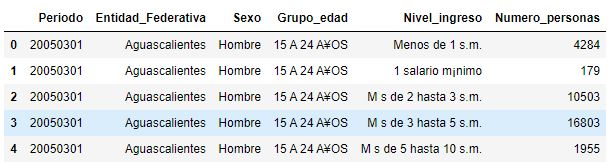
\includegraphics[width=1\linewidth]{Figure/InitialDataSet_Standarization.JPG}
	\caption{Fragmento del dataset utilizado sin procesar.}
	\label{fig:InitialDataSet}
\end{figure}

Con el objetivo de poder utilizar la informaci\'on fue necesario generar una estandarizaci\'on para las columnas, estados, espacio temporal. 
Las columnas se estandarizaron de la siguiente manera:


\begin{lstlisting}[language=Python]
data = pd.read_csv(data_path, encoding='latin1').rename(
    columns = {
        "Periodo": "t",
        "Entidad_Federativa": "state",
        "Sexo": "gender",
        "Grupo_edad": "age",
        "Nivel_ingreso": "wage_level",
        "Numero_personas": "population"
    }
)
\end{lstlisting}

Se detectaron las diferencias este los estados y unific\'o con el siguiente c\'odigo:

\begin{lstlisting}[language=Python]
# Standardize state variable
standardize_state = {
    'Coahuila': 'Coahuila de Zaragoza',
    'Ciudad de M\x82xico': 'Distrito Federal',
    'Estado de M\x82xico': 'M\'exico', 
    'Michoac\xa0n': 'Michoac\'an de Ocampo', 
    'Nuevo Le¢n': 'Nuevo Le\'on',
    'Queretaro': 'Quer\'etaro', 
    'San Luis Potos¡': 'San Luis Potos\'i', 
    'Veracruz': 'Veracruz de Ignacio de la Llave',
    'Yucat\xa0n': 'Yucat\'an'
}

data['state'] = [standardize_state.get(s, s) for s in data.state]
\end{lstlisting}

Se sigui\'o el mismo proceso con el resto de las variables dentro del dataset:
\begin{lstlisting}[language=Python]
# Standardize year variable
data['year'] = [int(str(y)[:4]) for y in data.t]

# Standardize age variable
standardize_age_dictionary = {age_val: age_val.replace("A¥OS", "").replace(" ", "") for age_val in data.age.unique()} 
data['age'] = [standardize_age_dictionary[age] for age in data.age]
\end{lstlisting}

De igual forma se limpiaron los datos de informcai\'on poco relevante para el estudio ('Nacional', No especificado, y NO ESPECIFICADO).

Campo estado ( ver figura \ref{fig:stateUnique_Standarization})

\begin{figure}[h!]
	\centering
	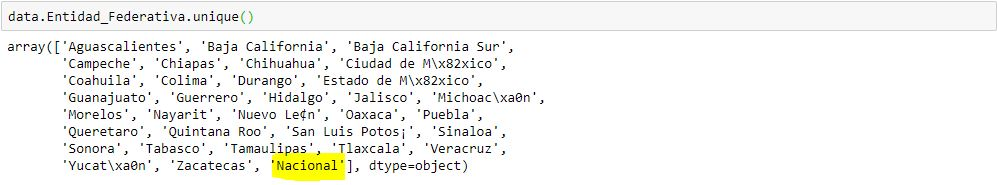
\includegraphics[width=1\linewidth]{Figure/stateUnique_Standarization.JPG}
	\caption{Valores que se limpiaron del dataset a trav\'es de la eliminaci\on de sus respectivas las filas}
	\label{fig:stateUnique_Standarization}
\end{figure}

Campo Salario ( ver figura \ref{fig:wageUnique_Standarization})
\begin{figure}[h!]
	\centering
	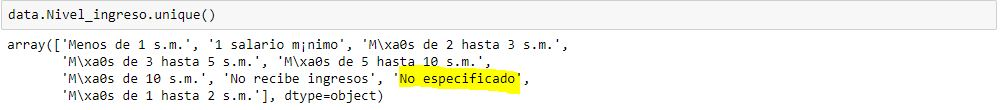
\includegraphics[width=1\linewidth]{Figure/wageUnique_Standarization.JPG}
	\caption{Valores que se limpiaron del dataset a trav\'es de la eliminaci\on de sus respectivas las filas}
	\label{fig:wageUnique_Standarization}
\end{figure}

Campo edad ( ver figura \ref{fig:ageUnique_Standarization})
\begin{figure}[h!]
	\centering
	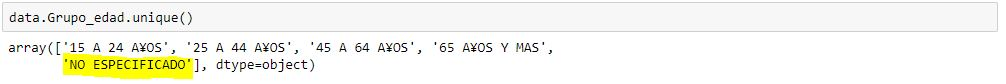
\includegraphics[width=1\linewidth]{Figure/ageUnique_Standarization.JPG}
	\caption{Valores que se limpiaron del dataset a trav\'es de la eliminaci\'on de sus respectivas las filas}
	\label{fig:ageUnique_Standarization}
\end{figure}

\subsubsection{Visualizaci\'on de los datos estandarizados}
Despues de estandarizar los datos 
\begin{figure}[h!]
	\centering
	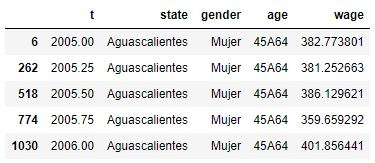
\includegraphics[width=0.8\linewidth]{Figure/AGSdatos_visualizacion.JPG}
	\caption{Datos usados para las graficas de las figuras} \ref{fig:AGSwageVSyear}, \ref{fig:AGSIncrementsVSyear} 
	\label{fig:AGSdatos}
\end{figure}

\begin{figure}[h!]
	\centering
	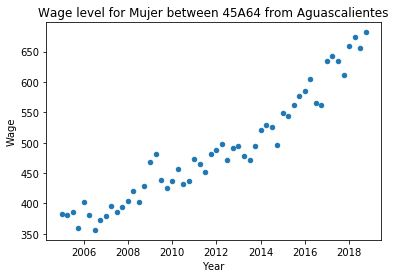
\includegraphics[width=0.8\linewidth]{Figure/AGSwageVSyear_visualizacionJPG.JPG}
	\caption{Salario en funcion del año usando un subconjunto de datos aleatorio} 
	\label{fig:AGSwageVSyear}
\end{figure}

\begin{figure}[h!]
	\centering
	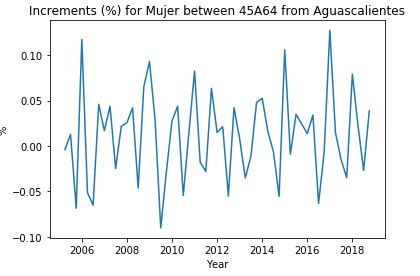
\includegraphics[width=0.8\linewidth]{Figure/AGSIncrementsVSyear_visualizacion.JPG}
	\caption{Incremento en funcion del año usando un subconjunto de datos aleatorio} 
	\label{fig:AGSIncrementsVSyear}
\end{figure}


\subsubsection{Autocorrelaci\'on Parcial}
Las gr\'aficas de autocorrelaci\'on y autocorrelaci\'on parcial se usan mucho en el an\'alisis y pron\'ostico de series de tiempo.
Estas son gr\'aficas que resumen gr\'aficamente la fuerza de una relaci\'on con una observaci\'on en una serie de tiempo con observaciones en pasos de tiempo anteriores. La diferencia entre la autocorrelaci\'on y la autocorrelaci\'on parcial puede ser dif\'icil y confusa para los principiantes con el pron\'ostico de series de tiempo.

Una autocorrelaci\'on parcial es un resumen de la relaci\'on entre una observaci\'on en una serie de tiempo con observaciones en pasos de tiempo anteriores con las relaciones de observaciones intermedias eliminadas.

La autocorrelaci\'on parcial en el retraso k es la correlaci\'on que resulta despu\'es de eliminar el efecto de cualquier correlaci\'on debido a los t\'erminos en los retrasos m\'as cortos.

La autocorrelaci\'on para una observaci\'on y una observaci\'on en un paso de tiempo anterior comprende tanto la correlaci\'on directa como las correlaciones indirectas. Estas correlaciones indirectas son una funci\'on lineal de la correlaci\'on de la observaci\'on, con observaciones en pasos temporales intermedios.

Son estas correlaciones indirectas las que la funci\'on de autocorrelaci\'on parcial busca eliminar. Sin entrar en las matem\'aticas, esta es la intuitivamente la autocorrelaci\'on parcial.

\begin{figure}[h!]
	\centering
	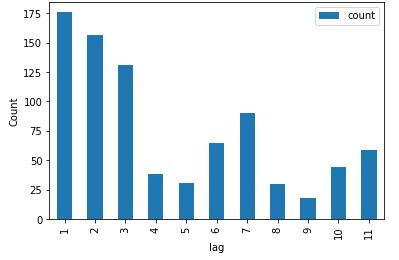
\includegraphics[width=0.8\linewidth]{Figure/Data_PartialAutocorrelation.JPG}
	\caption{Lag level per group} 
	\label{fig:LagLevel}
\end{figure}

\subsubsection{Generaci\'on del dataset de entrenamiento}
%%---------------------- Reempleazar
Lorem ipsum dolor sit amet, consectetur adipiscing elit, sed do eiusmod tempor incididunt ut labore et dolore magna aliqua. Ut enim ad minim veniam, quis nostrud exercitation ullamco laboris nisi ut aliquip ex ea commodo consequat. Duis aute irure dolor in reprehenderit in voluptate velit esse cillum dolore eu fugiat nulla pariatur. Excepteur sint occaecat cupidatat non proident, sunt in culpa qui officia deserunt mollit anim id est laborum.
%%---------------------
\begin{figure}[h!]
	\centering
	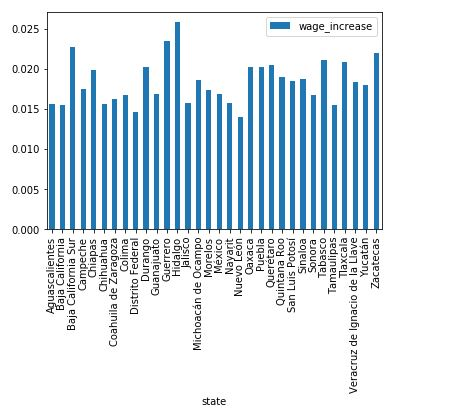
\includegraphics[width=0.8\linewidth]{Figure/Data_TrainingDataset.JPG}
	\caption{Lag level per group} 
	\label{fig:InitialData}
\end{figure}

%%---------------------- Reempleazar
Lorem ipsum dolor sit amet, consectetur adipiscing elit, sed do eiusmod tempor incididunt ut labore et dolore magna aliqua. Ut enim ad minim veniam, quis nostrud exercitation ullamco laboris nisi ut aliquip ex ea commodo consequat. Duis aute irure dolor in reprehenderit in voluptate velit esse cillum dolore eu fugiat nulla pariatur. Excepteur sint occaecat cupidatat non proident, sunt in culpa qui officia deserunt mollit anim id est laborum.
%%---------------------
\begin{figure}[h!]
	\centering
	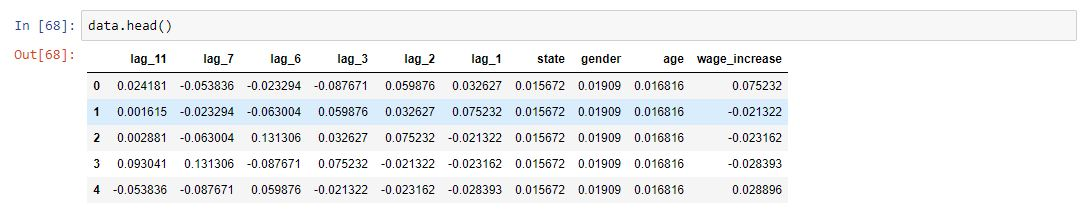
\includegraphics[width=1\linewidth]{Figure/DataSet_TrainingDataset.JPG}
	\caption{Lag level per group} 
	\label{fig:TrainingDataSet}
\end{figure}


\subsection{Descripci\'on del Modelo a Utilizar}

\subsubsection{Regresi\'on Lineal}

\subsubsection{Decision Tree}
Los modelos de \'arbol de Regresi\'on y Clasificaci\'on (C&RT, Classification & Regression Trees), fueron introducidos en la Estad\'istica por Breiman et al. (1984). Diversos autores utilizan el t\'ermino ``modelos de \'arbol de regresi\'on'' cuando la variable respuesta es cuantitativa y el de ``modelos de \'arbol de clasificaci\'o'' cuando \'esta es cualitativa. 
Decision tree Regression es un algoritmo de aprendizaje dentro del grupo de aprendizaje supervisado. Este se caracteriza por particionar o dividir los datos en varias clasificaciones de grupos homog\'eneos respecto a la variable, creando iteraciones de estas clasificaciones del DataFrame hasta conseguir el mejor resultado posible. Este m\'etodo utiliza los datos de entrenamiento de periodos anteriores y los entrena para conseguir clasificar los nuevos datos.
Dentro de las ventajas de este algoritmo se encuentran las siguientes:
Facilidad al comprender y explorar datos, debido a su clasificaci\'on y traficaci\'on. 
Dentro de las ventajas de este algoritmo se encuentran:
Los sobreajustes son muy comunes en estos modelos y al usar variables continuas, se tiene por sobre entendido que se perder\'a precisi\'on.

\subsubsection{Random Forest Regressor}


\subsubsection{XGBoost}
Es muy parecido al modelo Random Forest, pero esta vez los \'arboles tienen asociadas una funci\'on de p\'erdidas que tienen que minimizar (o maximizar) para conseguir los mejores resultados (por ello la palabra Boosting).
Est\'a basado o es muy parecido al \'arbol de decisi\'on y es una evoluci\'on entre la clasificaci\'on y la regresi\'on  este se basa en impulsar  para maximizar o minimizar la funci\'on de p\'erdidas trabaja sobre bases de datos de gran tamaño as\'i como m\'ultiples variables algo importante es que admite missing values  por lo mencionado anteriormente se debe tener en cuenta el equipo para  correr bases de datos extensas y usar muchas variables, es recomendable saber las variables que m\'as aportan al algoritmo.

Este clasifica o pron\'ostica sobre la variable objetivo, utiliza un set de datos utilizando los los \'arboles de decisiones para potencializar los resultados en base a un procesamiento secuencial y con una funci\'on de p\'erdida  que minimiza el error en consecuencia es un pronosticador fuerte. Como en todo algoritmo se deben ajustar los par\'ametros para obtener un m\'inimo error de precisi\'on


\subsection{Delimitaciones}
\subsubsection{Datos}
La serie estad\'istica presenta la poblaci\'on que tiene una actividad economica subordinada y remunerada del pais para cada una de las entidades federativas, desglosada por sexo, grupos de edad y cual es el nivel de ingreso de la poblaci\'on.\ref{fig:TrainingDataSet}\cite{datosAbiertos_2019}
\subsubsection{Temporales}
El presente es un estudio longitudinal en donde los datos de 2005 a 2018 se utilizar\'an como entrada para poder predecir el de salario, del 2019

%\subsubsection{Te\'oricas}
%----------------------------------------------------------------------------------------
%	Section 6
%----------------------------------------------------------------------------------------
\newpage
\section{Resultados}
\subsubsection{Regresi\'on Lineal}
Sin la introducci\'on de par\'ametros se alcanzo el 0.082 de sme:

\begin{figure}[h!]
	\centering
	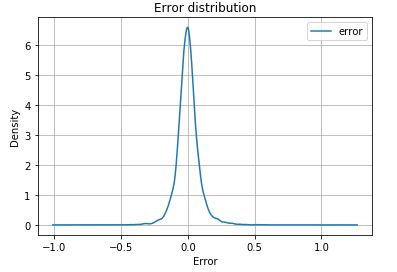
\includegraphics[width=0.8\linewidth]{Figure/LinearRegresionED_Results.JPG}
	\caption{Regresi\'on Lineal: distribuci\'on de error} 
	\label{fig:LinearRegresionED_Results}
\end{figure}

\begin{figure}[h!]
	\centering
	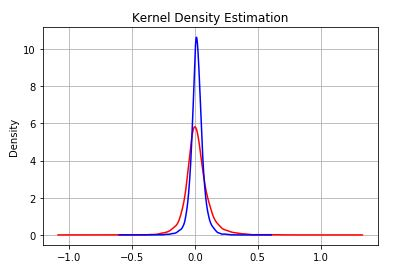
\includegraphics[width=0.8\linewidth]{Figure/LinearRegresionKernel_Results.JPG}
	\caption{Regresi\'on Lineal: Estimaci\'on de densidad del n\'ucleo} 
	\label{fig:LinearRegresionKernel_Results}
\end{figure}

\begin{figure}[h!]
	\centering
	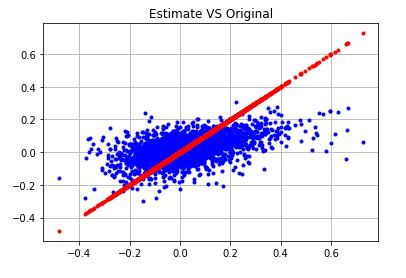
\includegraphics[width=0.8\linewidth]{Figure/RegresionLineal_Results.JPG}
	\caption{Regresi\'on Lineal: Estimate vs Original} 
	\label{fig:LinearRegresionKernel_Results}
\end{figure}
\\
\\
\newpage
\subsubsection{Decision Tree}
El mejor m\'odelo se obtuvo con los siguientes par\'ametros con un sme de 0.093583:
\begin{lstlisting}[language=Python]
{	'criterion': mae		
	'splitter': best	
	'max_depth':2.0		
	'max_features':0.24
}\end{lstlisting}
\\
Las siguientes gr\'aficas corresponden a los resultados con los respectivos par\'ametros y usando los set de pruebas:
\begin{figure}[h!]
	\centering
	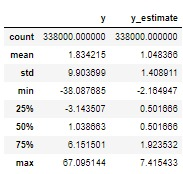
\includegraphics[width=0.3\linewidth]{Figure/dtr_decription.jpeg}
	\caption{Data description (DT)} 
	\label{fig:dt_ed}
\end{figure}
\\
\begin{figure}[h!]
	\centering
	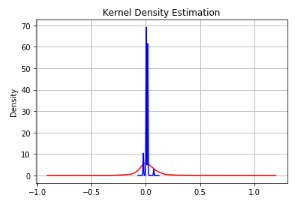
\includegraphics[width=0.8\linewidth]{Figure/dtr_kerneldensity.jpeg}
	\caption{Kernel density (DT)} 
	\label{fig:dt_kd}
\end{figure}
\\
\begin{figure}[h!]
	\centering
	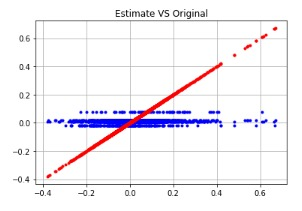
\includegraphics[width=0.8\linewidth]{Figure/dtr_estimorg.jpeg}
	\caption{Estimate vs Original(DT)} 
	\label{fig:dt_eo}
\end{figure}

\newpage
\subsubsection{XGBoost}
El mejor m\ódelo se obtuvo con los siguientes par\'ametros con un sme de 0.062:
\begin{lstlisting}[language=Python]
xgb_grid.best_params_
{'colsample_bytree': 0.7, 
'learning_rate': 0.07, 
'max_depth': 5, 
'min_child_weight': 4, 
'n_estimators': 100, 
'nthread': 4, 
'objective': 'reg:linear', 
'silent': 1, 
'subsample': 0.7}
\end{lstlisting}
Las siguientes gr\'aficas corresponden a los resultados con los respectivos par\'ametros y usando los set de pruebas:
\begin{figure}[h!]
	\centering
	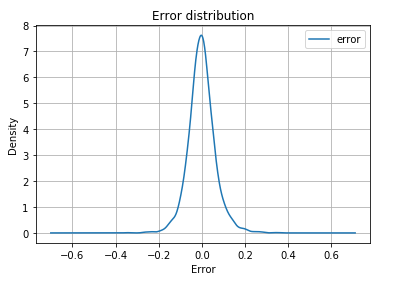
\includegraphics[width=0.8\linewidth]{Figure/xgbregresor_results.png}
	\caption{Error distribution(XGB)} 
	\label{fig:xgbregresor}
\end{figure}
\begin{figure}[h!]
	\centering
	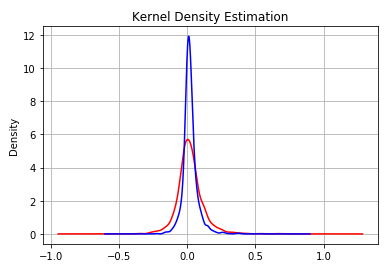
\includegraphics[width=1\linewidth]{Figure/xgbregresorKernel_results.png}
	\caption{Error distribution(XGB)} 
	\label{fig:xgbregresorKernel_results}
\end{figure}
\begin{figure}[h!]
	\centering
	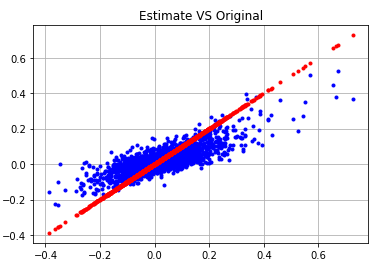
\includegraphics[width=0.8\linewidth]{Figure/xgbregresorEstimation_results.png}
	\caption{Error distribution(XGB)} 
	\label{fig:xgbregresorEstimation_results}
\end{figure}
\\
\\
\newpage
\subsubsection{Naive Bayes}
Best parameter:
smoothing: 307

Las siguientes gr\'aficas corresponden a los resultados con los respectivos par\'ametros y usando los set de pruebas:
\begin{figure}[h!]
	\centering
	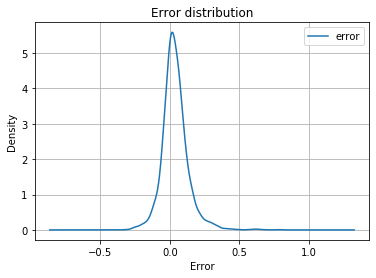
\includegraphics[width=0.8\linewidth]{Figure/nb_error_distribution.png}
	\caption{Error Distribution (Naive Bayes)} 
	\label{fig:nb1}
\end{figure}

\begin{figure}[h!]
	\centering
	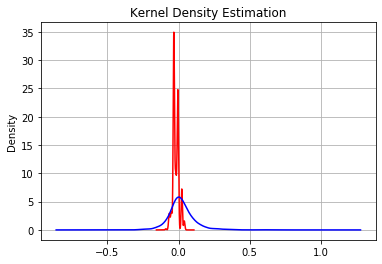
\includegraphics[width=0.8\linewidth]{Figure/nb_density_estimation.png}
	\caption{Density Estimation (Naive Bayes)} 
	\label{fig:nb1}
\end{figure}

\begin{figure}[h!]
	\centering
	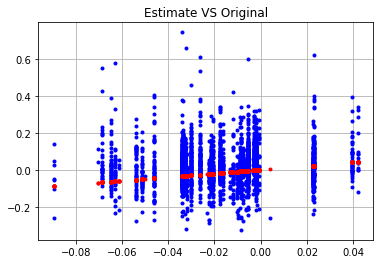
\includegraphics[width=0.8\linewidth]{Figure/nb_estimate_vs_original.png}
	\caption{Estimation vs Original (Naive Bayes)} 
	\label{fig:nb1}
\end{figure}\\

\newpage
\subsubsection{Support Vector Machines Regressor}
\p{El mejor m\'odelo se obtuvo con los siguientes par\'ametros con un sme de 0.093:
\begin{lstlisting}[language=Python]
{'kernel':'poly', 
 'degree':'2', 
 'gamma':'0.55', 
 'coef0':'0.1', 
 'C':'34', 
 'epsilon':'0.2'
}
\end{lstlisting}{}
Las siguientes gr\'aficas corresponden a los resultados con los respectivos par\'ametros y usando los set de pruebas:
\begin{figure}[h!]
	\centering
	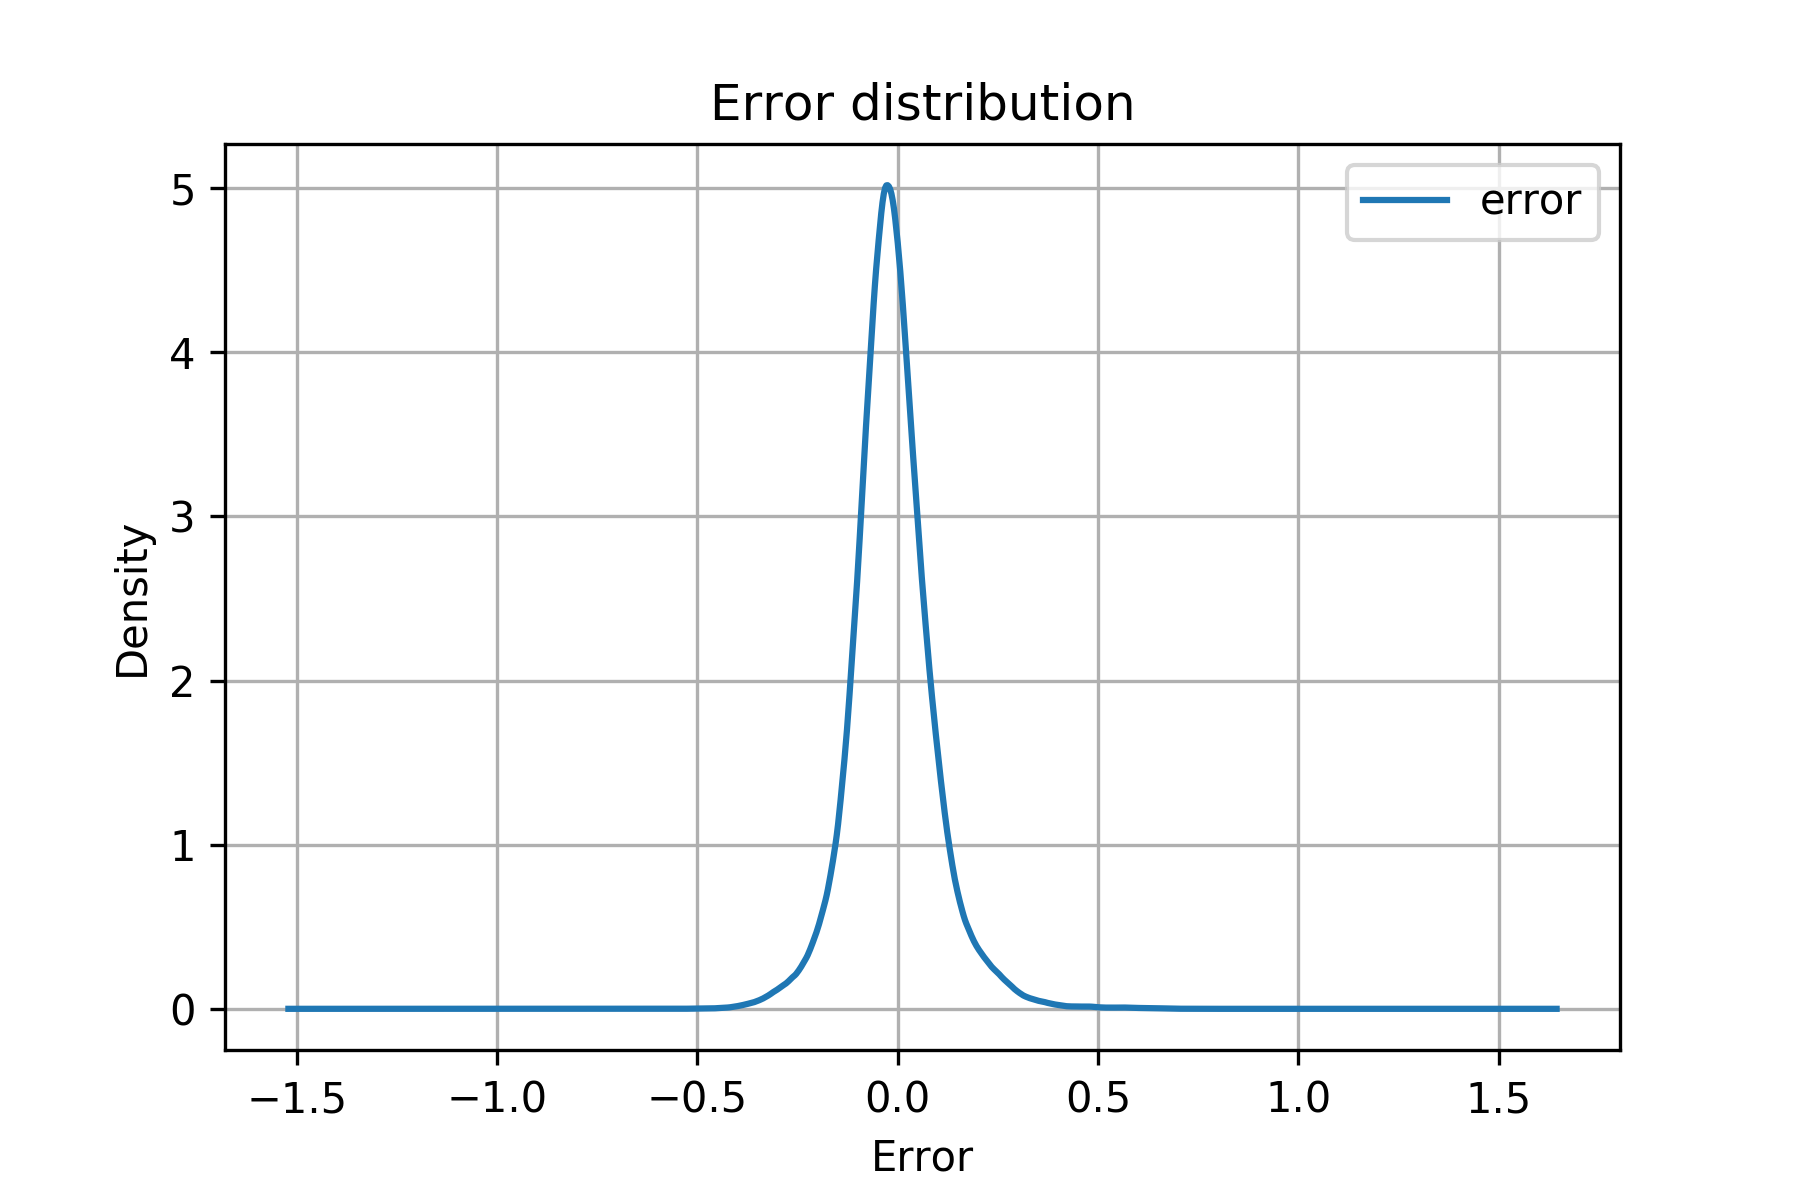
\includegraphics[width=0.8\linewidth]{Figure/svmr_errordist.png}
	\caption{Error Distribution (SVMR)} 
	\label{fig:svmr_ed}
\end{figure}

\begin{figure}[h!]
	\centering
	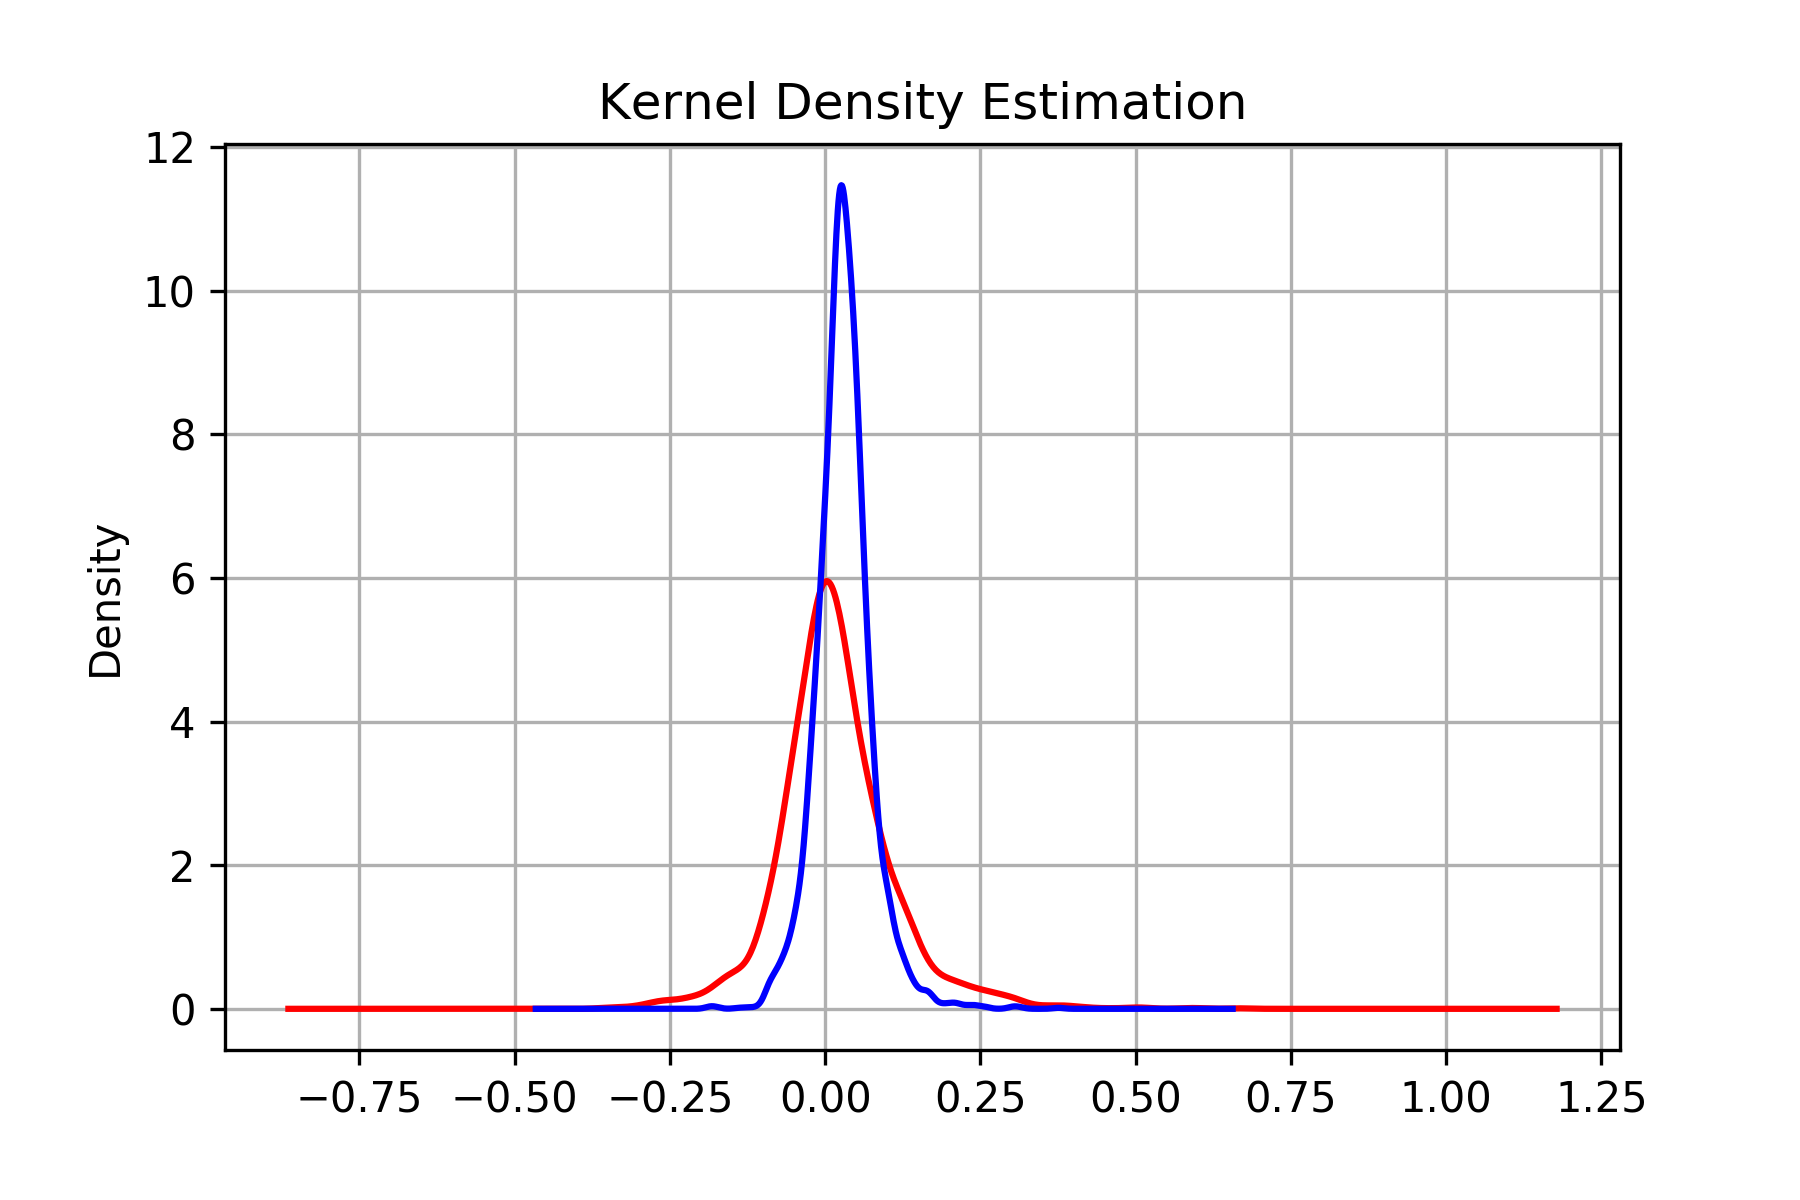
\includegraphics[width=0.8\linewidth]{Figure/svmr_kerneldensity.png}
	\caption{Kernel density (SVMR)} 
	\label{fig:svmr_kd}
\end{figure}

\begin{figure}[h!]
	\centering
	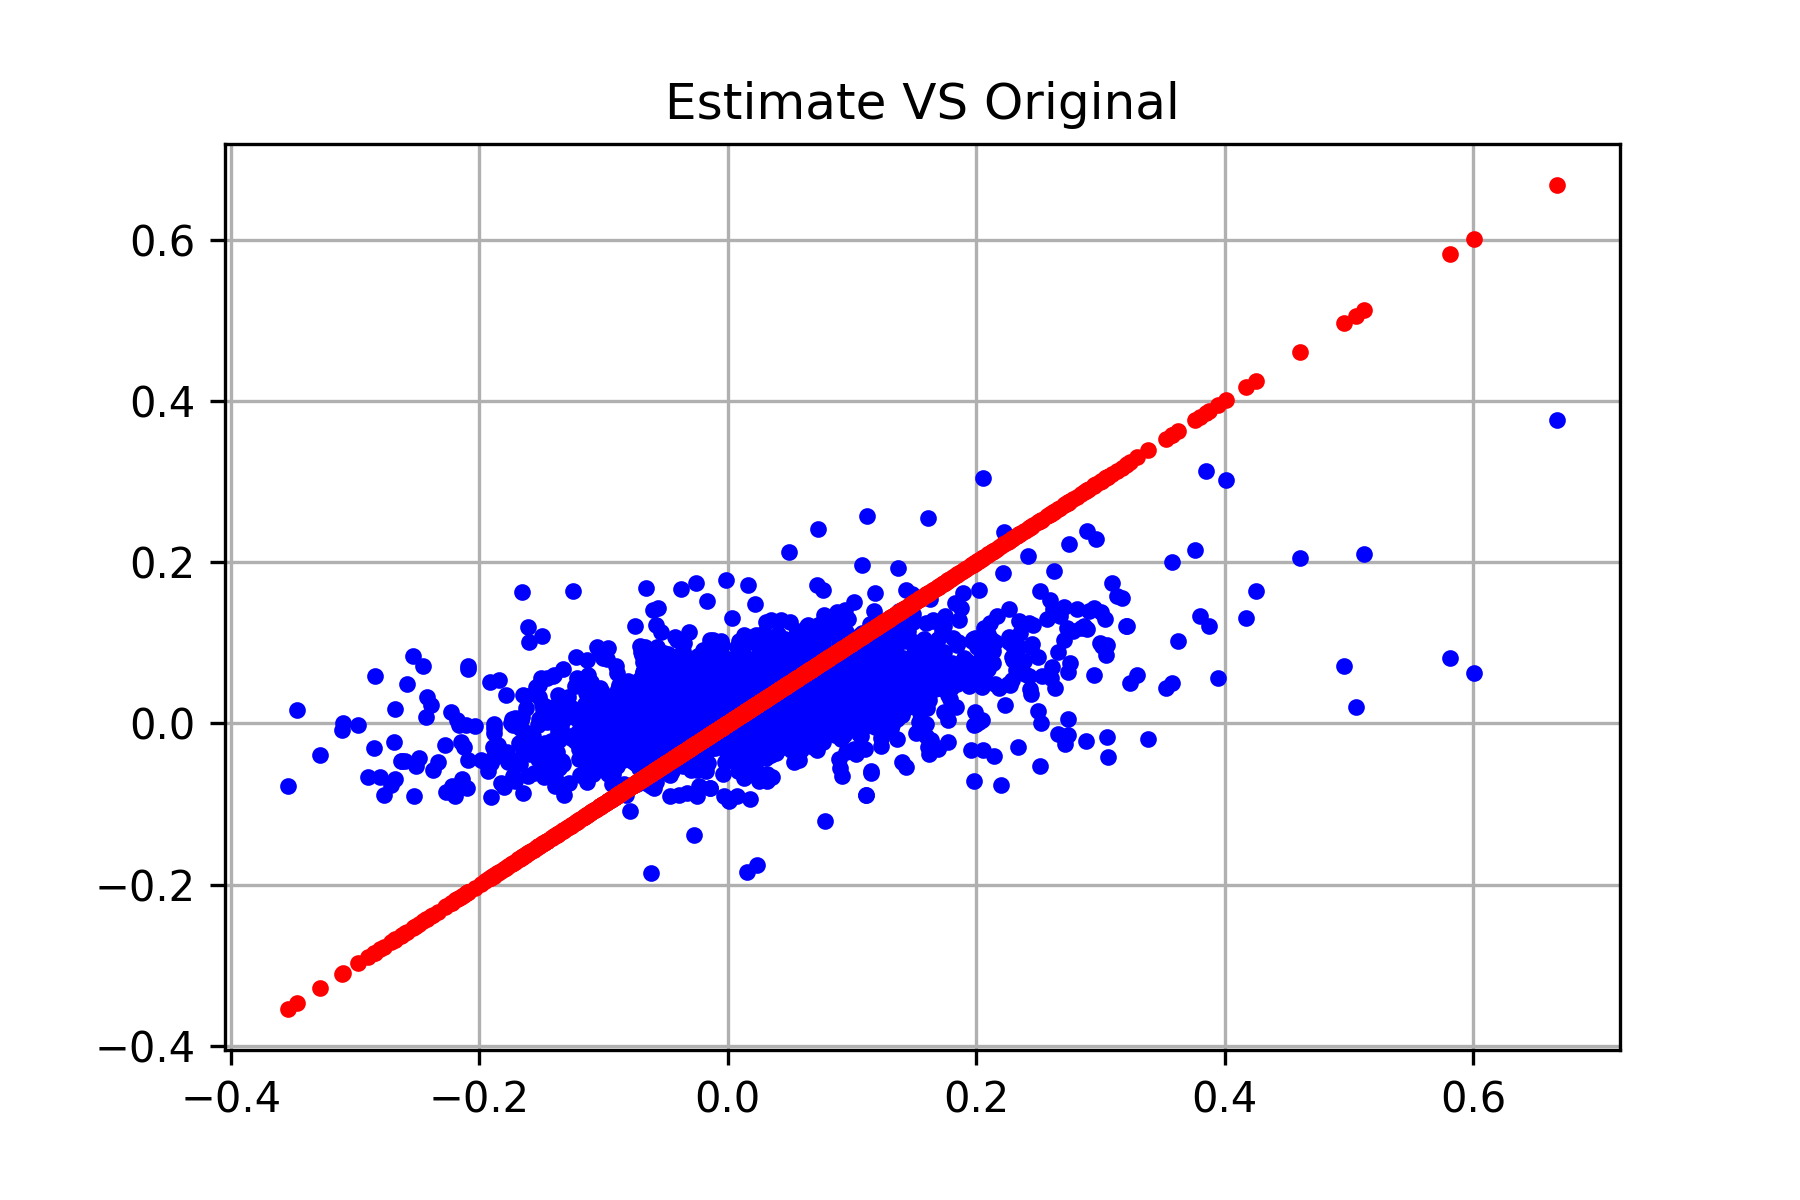
\includegraphics[width=1\linewidth]{Figure/svmr_estiorg.png}
	\caption{Estimate vs Original(SVMR)} 
	\label{fig:svmr_eo}
\end{figure}
} \\

\newpage
%----------------------------------------------------------------------------------------
%	Section 7
%----------------------------------------------------------------------------------------
\newpage
\newpage
\section{Conclusiones}

%%---------------------- Reempleazar
Lorem ipsum dolor sit amet, consectetur adipiscing elit, sed do eiusmod tempor incididunt ut labore et dolore magna aliqua. Ut enim ad minim veniam, quis nostrud exercitation ullamco laboris nisi ut aliquip ex ea commodo consequat. Duis aute irure dolor in reprehenderit in voluptate velit esse cillum dolore eu fugiat nulla pariatur. Excepteur sint occaecat cupidatat non proident, sunt in culpa qui officia deserunt mollit anim id est laborum.
%%---------------------

%bibliography
\newpage
\bibliographystyle{abbrv}
\bibliography{sample.bib}

\end{document}